\documentclass{exam}

\usepackage{graphicx} %for images
\pagenumbering{gobble}
\usepackage{titling}
\setlength{\droptitle}{-8ex}
\pretitle{\begin{flushleft}\Large\bfseries}
\posttitle{\par\end{flushleft}}
\preauthor{\begin{flushleft}\Large}
\postauthor{\end{flushleft}}
\predate{\begin{flushleft}}
\postdate{\end{flushleft}}
\usepackage{enumerate} %for alphabetized lists
\usepackage{amsmath}
\usepackage{multicol} %for multiple columns
\usepackage{systeme} %systems of equations
\renewcommand{\questionshook}{\setlength{\itemsep}{15pt}} %controls space betweenites

\usepackage{listings} %for programming snippets
\usepackage{color} %for keyword colors in programming snippets
%the following is for java listings
\definecolor{dkgreen}{rgb}{0,0.6,0}
\definecolor{gray}{rgb}{0.5,0.5,0.5}
\definecolor{mauve}{rgb}{0.58,0,0.82}
\lstset{%frame=tblr,
  language=Java,
  aboveskip=3mm,
  belowskip=3mm,
  showstringspaces=false,
  columns=flexible,
  basicstyle={\small\ttfamily},
  numbers=none,
  numberstyle=\tiny\color{gray},
  keywordstyle=\color{blue},
  commentstyle=\color{dkgreen},
  stringstyle=\color{mauve},
  breaklines=true,
  breakatwhitespace=true,
  tabsize=3
}




%fromhttps://texblog.org/2012/06/25/adding--lines--for--taking--handwritten--notes--in--latex/
\usepackage{pgffor, ifthen}
\newcommand{\notes}[3][\empty]{%q
   vspace{10pt}\\
    \foreach \n in {1,...,#2}{%
        \ifthenelse{\equal{#1}{\empty}}
            {\rule{#3}{0.5pt}\\}
            {\rule{#3}{0.5pt}\vspace{#1}\\} 
        }
}

\title{Free Response Question: ArrayLists}

\author{  }


\begin{document}
\maketitle
%\thispagestyle{empty}
\noindent This question involves the creation of user names for an online system. A user name is created based on a user's first and last names. A new user name cannot be a duplicate of a user name already assigned. You will write the constructor and one method of the \texttt{UserName} class. A partial declaration of the \texttt{UserName}  class is shown below.





\begin{lstlisting}

public class UserName
{
// The list of possible user names, based on a user's first and last names and initialized by the constructor.
private ArrayList<String> possibleNames;
 
/** Constructs a UserName object as described in part (a).
* Precondition: firstName and lastName have length greater than 0
* and contain only uppercase and lowercase letters.
*/
public UserName(String firstName, String lastName)
{ /* to be implemented in part (a) */ }
 
/** Returns true if arr contains name, and false otherwise. */
public boolean isUsed(String name, String[] arr)
{ /* implementation not shown */ }
 
/** Removes strings from possibleNames that are found in usedNames as described in part (b).
*/
public void setAvailableUserNames(String[] usedNames)
{ /* to be implemented in part (b) */ }
}
\end{lstlisting}
\newpage
\begin{questions}
\question

Write the constructor for the \texttt{UserName}  class. The constructor initializes and fills \texttt{possibleNames}  with possible user names based on the  \texttt{firstName} and  \texttt{lastName} parameters. The possible user names are obtained by concatenating  \texttt{lastName} with different substrings of  \texttt{firstName}. The substrings begin with the first character of  \texttt{firstName} and the lengths of the substrings take on all values from 1 to the length of  \texttt{firstName}.

The following example shows the contents of possibleNames after a  \texttt{UserName} object has been instantiated.\\

\underline{Example}

 \texttt{UserName person = new UserName("john", "smith");}

After the code segment has been executed, the possibleNames instance variable of person will contain the following String objects in some order.

 \texttt{"smithj", "smithjo", "smithjoh", "smithjohn"}\\

Write the  \texttt{UserName} constructor below:

\begin{lstlisting}
/** Constructs a UserName object as described in part (a).
* Precondition: firstName and lastName have length greater than 0
* and contain only uppercase and lowercase letters.
*/
public UserName(String firstName, String lastName)

\end{lstlisting}
\makeemptybox{\stretch{1}}
\newpage
\question
Write the \texttt{UserName} method \texttt{setAvailableUserNames}. The method removes from \texttt{possibleNames} all names that are found in \texttt{usedNames}. These represent user names that have already been assigned in the online system and are therefore unavailable.

A helper method, \texttt{isUsed}, has been provided. The \texttt{isUsed} method searches for name in \texttt{arr.} The method returns true if an exact match is found and returns false otherwise.

The example below shows the intended behavior of the \texttt{setAvailableUserNames} method.

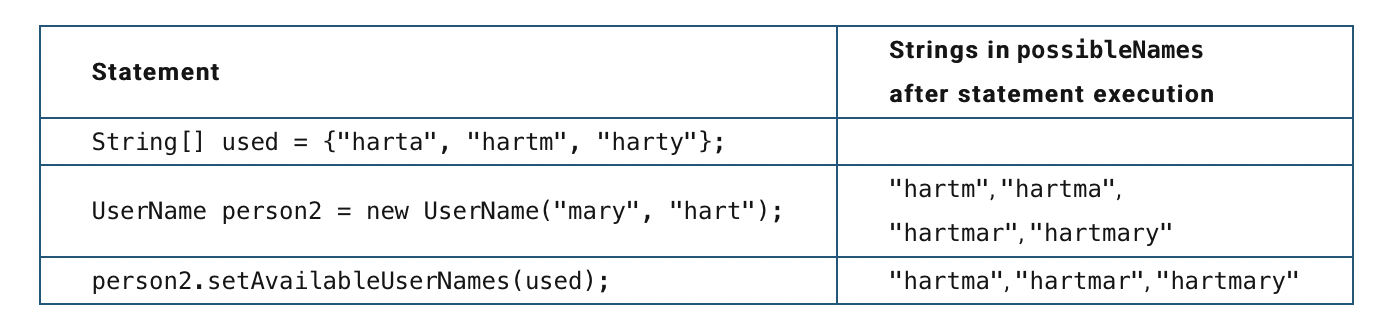
\includegraphics[scale=0.5]{table.png}


Complete the  \texttt{setAvailableUserNames} method below.
\begin{lstlisting}
/** Removes strings from possibleNames that are found in usedNames as described in part (b).
*/
public void setAvailableUserNames(String[] usedNames)
\end{lstlisting}
\makeemptybox{\stretch{1}}
\end{questions}


\end{document}